\documentclass[11pt]{article}
\usepackage[margin=1in]{geometry}
\usepackage{graphicx}
\usepackage{booktabs}
\usepackage{xcolor}
\usepackage{hyperref}
\usepackage{amsmath}
\usepackage{listings}
\usepackage{enumitem}
\usepackage{caption}
\usepackage{float}
\usepackage{longtable}

\hypersetup{colorlinks=true, linkcolor=blue, urlcolor=blue, citecolor=blue}

\definecolor{codebg}{rgb}{0.96,0.96,0.96}
\lstset{
  basicstyle=\ttfamily\small,
  backgroundcolor=\color{codebg},
  frame=single,
  breaklines=true,
  columns=fullflexible,
  keywordstyle=\color{blue!70!black}\bfseries,
  commentstyle=\color{green!40!black}\itshape,
  stringstyle=\color{orange!70!black},
  language=C++,
  tabsize=2,
}

\title{\Large\textbf{Lab Assignment Report: Medium Access Control ---\\ CSMA Techniques with Collision Detection}}
\author{Sajjad Ahmed Shaaz \\ 002410501093 \\ BCSE-III A3}
\date{September 28, 2026}

\begin{document}
\maketitle

\section*{Basic Information}
\begin{itemize}[leftmargin=1.6em]
  \item \textbf{Subject:} CSE/PC/B/S/314 Computer Networks Lab
  \item \textbf{Assignment Number:} 3
  \item \textbf{Problem Statement:} Design and implement medium access control mechanisms
  within a simulated network environment using IEEE 802 standards: Non-Persistent CSMA,
  1-Persistent CSMA, $p$-Persistent CSMA, and CSMA/CD. An emulated shared channel maintains
  its state (IDLE / BUSY / COLLISION) while independent client processes, each modeling one
  network station, sense the channel and attempt transmission according to the strategy
  under test.
  \item \textbf{Code demonstration due:} 21--25 September 2026 \quad
  \textbf{Report submission due:} next lab classes
\end{itemize}

\section{Design}

\subsection{Purpose of the Program}
Assignments 1 and 2 operated one sender and one receiver at a time. This assignment moves
one layer down the stack, to the problem that exists only when \emph{more than one} station
wants the same physical medium at once: how does a station decide when it is safe to
transmit, and what does it do when it guesses wrong and collides with another station? Four
carrier-sense strategies are implemented end-to-end on a shared emulated channel and
compared under identical, controlled contention so that their textbook trade-offs --- idle
time wasted being cautious, collision frequency from being aggressive, and the cost of a
collision once it happens --- are measured directly rather than only asserted.

\subsection{Design Rationale}
\paragraph{Slotted, lock-step channel.} A real multi-process CSMA simulation where every
station's socket writes race against each other in true continuous time would make the
outcome of ``simultaneous'' transmission a function of OS scheduling jitter rather than of
the protocol being tested --- and would be irreproducible. Instead, the channel is modeled
in discrete \emph{slots} (the standard approximation used to analyze CSMA/CD, where one slot
equals $2\times$ the propagation delay: the minimum time for a station to learn the medium
is occupied). The \texttt{channel\_server} drives every station through the same slot in
lock-step --- broadcast the sensed state, collect every station's action, resolve the
outcome --- so a collision is a deterministic fact (two or more stations chose
\texttt{TRANSMIT} in the same slot), not a race condition.

\paragraph{Saturated (backlogged) traffic.} The assignment asks how the number of
contending stations affects collisions, delay, and throughput --- not how offered load does.
Every station is therefore modeled as always having a frame ready to send: the moment one
frame is delivered, the next is immediately ready. This is the standard \emph{saturation
throughput} model used to characterize a MAC protocol's ceiling behavior, and it isolates
$N$ (and $p$) as the only free variables, exactly as the test cases require.

\paragraph{One shared backoff rule across all four schemes.} On a real collision, every
scheme needs \emph{some} random recovery mechanism, or two persistently-sensing stations
would simply re-collide forever in lock-step the instant the channel frees up. All four
schemes here use the identical IEEE 802.3 binary exponential backoff after a collision. This
is a deliberate control: it isolates the \emph{idle/busy sensing rule} (non-persistent vs.\
1-persistent vs.\ $p$-persistent vs.\ CD's early abort) as the only thing that differs
between schemes, so that a measured difference in the results is attributable to the
persistence strategy itself.

\paragraph{An omniscient channel server for statistics.} Because the server observes every
station's action every slot, it can compute each frame's delay (slots from when it became
ready to when it was successfully delivered) and the aggregate collision/throughput counters
directly, without extra reporting traffic from the stations --- mirroring how a real testbed
or network analyzer would instrument the medium from outside.

\subsection{Protocol Between Channel Server and Station}
Table~\ref{tab:protocol} lists the three message types exchanged every slot (Figure~\ref{fig:arch}).
Communication uses TCP (reliable, ordered) purely as the coordination transport for this
lock-step handshake --- it plays no role in the contention being modeled, which is entirely
at the application-logic level (deciding whether to send \texttt{TRANSMIT} or \texttt{WAIT}
in a given slot).

\begin{table}[H]
\centering
\begin{tabular}{llp{7.3cm}}
\toprule
\textbf{Direction} & \textbf{Message} & \textbf{Purpose} \\
\midrule
Server $\to$ Station & \texttt{SLOT n STATE} & Sensed channel state (IDLE/BUSY) for slot $n$ \\
Station $\to$ Server & \texttt{ACT n TRANSMIT\textbar WAIT} & This station's decision for slot $n$ \\
Server $\to$ Station & \texttt{OUTCOME SUCCESS\textbar COLLISION} & Resolution of \emph{this station's own} in-flight frame (never broadcast to bystanders, since a station cannot itself detect a collision it is not party to) \\
Server $\to$ Station & \texttt{DONE} & Simulation horizon reached \\
\bottomrule
\end{tabular}
\caption{Wire protocol between \texttt{channel\_server} and each \texttt{station}.}
\label{tab:protocol}
\end{table}

\begin{figure}[H]
\centering
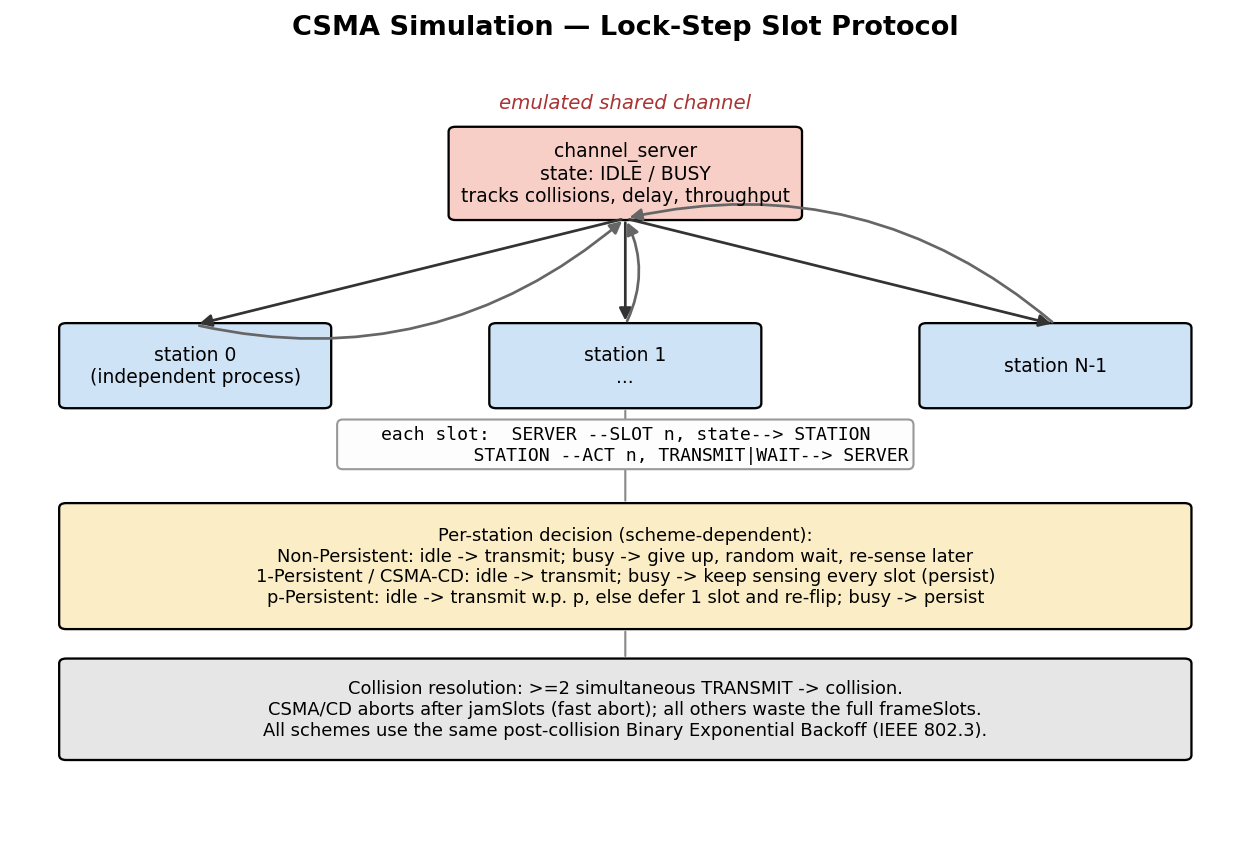
\includegraphics[width=0.92\textwidth]{figures/architecture.png}
\caption{Procedural structure: the channel server coordinates $N$ independent station
processes in lock-step time slots.}
\label{fig:arch}
\end{figure}

\subsection{Input and Output Format}
\textbf{Input:} \texttt{channel\_server} takes a port, station count $N$, scheme, $p$,
frame duration (in slots), CSMA/CD jam-detection window (in slots), and the simulation
horizon (total slots); each \texttt{station} takes the server's address/port, the same
scheme and $p$, and the backoff cap. \textbf{Output:} both endpoints log a human-readable
run summary to \texttt{stderr}; \texttt{channel\_server} additionally prints one
\texttt{RESULT,...} CSV line to \texttt{stdout} (scheme, $N$, $p$, frame/jam/max slots,
successes, collisions, idle slots, average delay, throughput) that
\texttt{run\_experiments.py} collects into \texttt{results/*.csv}.

\section{Implementation}
The project is implemented in C++17 with POSIX TCP sockets, plus a Python orchestration
script for the parameter sweeps.

\subsection{Component Breakdown}
\begin{itemize}[leftmargin=1.6em]
  \item \texttt{channel\_server.cpp} --- the emulated shared channel: runs the slot loop,
  resolves collisions vs.\ successes, computes all statistics.
  \item \texttt{station.cpp} --- one independent OS process per contending station;
  implements all four persistence strategies and the shared backoff rule.
  \item \texttt{common/protocol.h} --- message format and the \texttt{CsmaScheme} enum
  shared by both binaries.
  \item \texttt{common/net\_util.h} --- a buffered newline-delimited \texttt{LineSocket}
  over a blocking TCP connection.
  \item \texttt{run\_experiments.py} --- spawns a \texttt{channel\_server} + $N$
  \texttt{station} processes per configuration, parses the \texttt{RESULT} line, and
  aggregates \texttt{results/*.csv} for both required sweeps.
\end{itemize}

\subsection{Per-Slot Station Decision Logic}
Figure~\ref{fig:slottimeline} contrasts how a collision is resolved with and without
collision detection. The core per-slot decision (station side) is:
\begin{lstlisting}
if (awaitingOutcome)                 action = WAIT;             // our frame is in flight
else if (backoffRemaining > 0)       { backoffRemaining--; action = WAIT; }
else switch (scheme) {
    case NON_PERSISTENT:
        if (state == IDLE) action = TRANSMIT;
        else { backoffRemaining = uniform(1, 8); action = WAIT; }   // give up, don't persist
        break;
    case ONE_PERSISTENT:
    case CSMA_CD:
        action = (state == IDLE) ? TRANSMIT : WAIT;                 // keep sensing every slot
        break;
    case P_PERSISTENT:
        if (state == IDLE) action = (uniform01() < p) ? TRANSMIT : WAIT;
        else action = WAIT;                                          // persist, then re-flip
        break;
}
\end{lstlisting}
On \texttt{OUTCOME COLLISION} (any scheme), the station applies binary exponential backoff:
\begin{lstlisting}
collisionCount++;
int window = 1 << min(collisionCount, backoffCap);
backoffRemaining = uniform(0, window - 1);
\end{lstlisting}
The only scheme-specific behavior in collision \emph{cost} lives on the server: CSMA/CD
resolves a collision after \texttt{jamSlots} (a short, fixed abort window), while the other
three schemes --- lacking collision detection --- only discover the failure once the full
\texttt{frameSlots} duration has elapsed, exactly as on a real pre-802.3 CSMA link.

\begin{figure}[H]
\centering
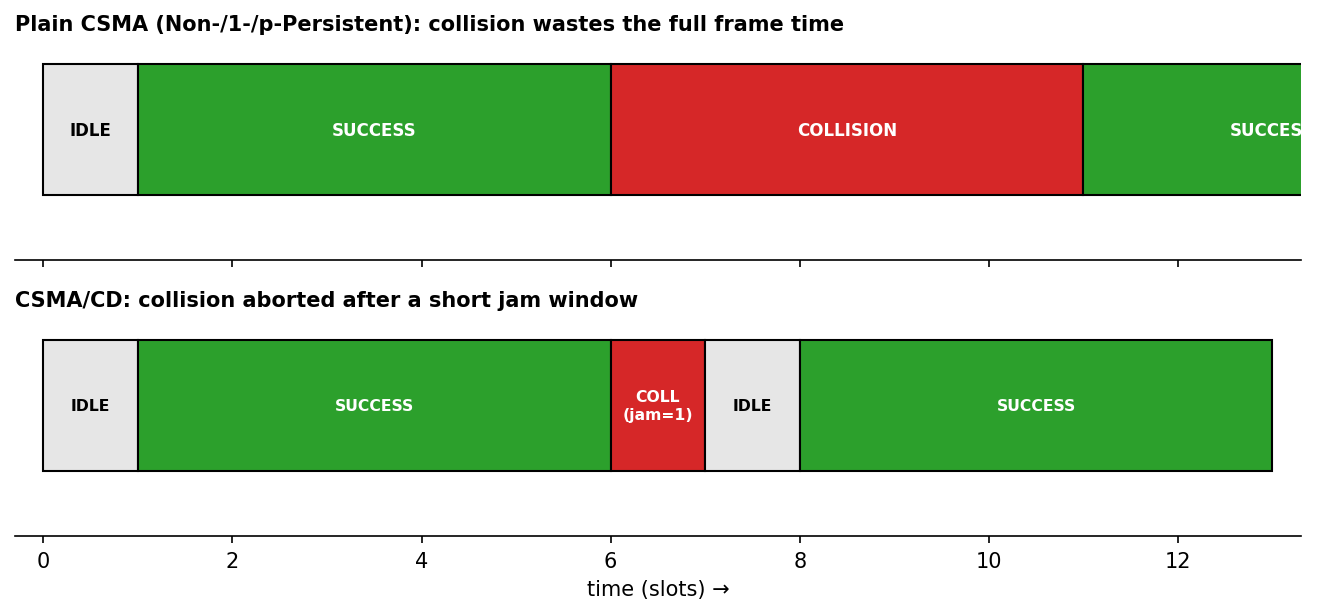
\includegraphics[width=\textwidth]{figures/slot_timeline.png}
\caption{Collision cost with vs.\ without collision detection, drawn to scale for
\texttt{frameSlots=5}, \texttt{jamSlots=1}.}
\label{fig:slottimeline}
\end{figure}

\subsection{Performance Metrics}
\begin{itemize}[leftmargin=1.6em]
  \item \textbf{Collisions} --- count of slot-groups in which $\ge 2$ stations chose
  \texttt{TRANSMIT} simultaneously (one event per group, regardless of how many stations
  were involved).
  \item \textbf{Average delay} (slots) --- for every successfully delivered frame, the
  number of slots between the frame becoming ready and its successful completion, averaged
  over all successful frames system-wide. Computed entirely server-side from
  \texttt{readySlot[stationId]}, which is reset to the completion slot immediately after
  each success (saturated model: the next frame is ready right away).
  \item \textbf{Normalized throughput} $S = \dfrac{\text{successes} \times
  \text{frameSlots}}{\text{maxSlots}}$ --- the fraction of total simulated time the channel
  spent carrying a successfully delivered frame; the standard metric in Kleinrock/Tobagi-style
  CSMA throughput analysis, bounded in $[0,1]$.
\end{itemize}

\section{Test Cases}
\begin{itemize}[leftmargin=1.6em]
  \item \textbf{TC1 --- Slot accounting is exact:} for any run,
  $\text{successes}\times\text{frameSlots} + \text{collisions}\times(\text{frameSlots or
  jamSlots}) + \text{idleSlots} = \text{maxSlots}$ (up to at most \texttt{frameSlots}$-1$
  from one transmission still in flight when the horizon is reached). \emph{Checking:} a
  first implementation failed this check by 331 slots out of 2000 (\S5.3); after the fix,
  every run in the results below balances exactly.
  \item \textbf{TC2 --- Minimal contention, $N{=}2$:} all four schemes should behave nearly
  identically and near-optimally, since two backlogged stations rarely both sense idle in
  the same slot. \emph{Checking:} throughput $\ge 0.98$ for every scheme at $N{=}2$
  (Table~\ref{tab:throughputN}).
  \item \textbf{TC3 --- CSMA/CD's collision cost is strictly cheaper:} with
  \texttt{jamSlots}$=1 \ll$ \texttt{frameSlots}$=5$, a collision under CSMA/CD should cost
  $5\times$ less channel time than under the other three schemes. \emph{Checking:} at high
  $N$ (Table~\ref{tab:throughputN}, $N{=}100$), CSMA/CD sustains throughput 0.739 versus
  $\approx 0.26$ for the non-CD schemes despite a \emph{higher} raw collision count (\S5).
  \item \textbf{TC4 --- Non-persistent defers instead of persisting:} when the channel is
  busy, a non-persistent station must not re-attempt every slot. \emph{Checking:} inspected
  station-side logs confirm a random multi-slot gap between a sensed-busy event and the next
  transmit attempt, unlike 1-persistent/CSMA-CD which attempt on the very next idle slot.
  \item \textbf{TC5 --- $p$-persistent degenerates correctly at the extremes:} $p{=}1$
  should behave like 1-persistent (always transmit when idle); very low $p$ should transmit
  rarely. \emph{Checking:} Table~\ref{tab:expA} shows $p{=}1.0$ throughput (0.766) close to
  1-persistent's $N{=}15$ throughput in Table~\ref{tab:throughputN} (0.782), and $p{=}0.05$
  shows the highest idle-slot count of the sweep (3110 of 20000).
  \item \textbf{TC6 --- $p$-sweep at fixed $N$ (required test case i):} $p \in
  \{0.05,\dots,1.0\}$, $N{=}15$ fixed. \emph{Checking:} collisions, delay, and throughput
  all vary non-monotonically with $p$ (\S4.1), matching the classic trade-off between
  excess deferral (low $p$) and excess collision (mid $p$).
  \item \textbf{TC7 --- All-schemes sweep across $N$ (required test case ii):} $N \in
  \{2,5,10,15,20,30,40,60,80,100\}$ for all four schemes, $p$-persistent at the best $p$
  from TC6. \emph{Checking:} every scheme's throughput is monotonically non-increasing in
  $N$ (\S4.2); no run hung or crashed across all 52 configurations.
  \item \textbf{TC8 --- No process hangs at high concurrency:} $N{=}100$ station processes
  connecting to one server. \emph{Checking:} completed in $\approx$6--10\,s per run with
  correct slot accounting; no deadlocks in the lock-step protocol.
\end{itemize}

\section{Results}

\subsection{Experiment A --- $p$-Persistent CSMA, Sweep $p$ (Fixed $N=15$)}
\label{sec:expA}

\begin{table}[H]
\centering
\small
\begin{tabular}{rrrr}
\toprule
\textbf{$p$} & \textbf{Collisions} & \textbf{Avg. Delay (slots)} & \textbf{Throughput $S$} \\
\midrule
0.05 & 1044 & 127.89 & 0.5835 \\
0.10 & 1563 & 141.45 & 0.5165 \\
0.15 & 1742 & 143.09 & 0.4910 \\
0.20 & 1818 & 143.04 & 0.4805 \\
0.30 & 1866 & 150.98 & 0.4743 \\
0.40 & 1879 & 151.78 & 0.4705 \\
0.50 & 1878 & 137.88 & 0.4743 \\
0.60 & 1816 & 140.04 & 0.4913 \\
0.70 & 1802 & 131.81 & 0.4965 \\
0.80 & 1743 & 135.81 & 0.5162 \\
0.90 & 1379 & 104.12 & 0.6135 \\
1.00 & 855  & 78.77  & 0.7660 \\
\bottomrule
\end{tabular}
\caption{Experiment A: $p$-Persistent CSMA, $N=15$, \texttt{frameSlots}$=5$,
\texttt{maxSlots}$=20000$. Best throughput at $p=1.0$.}
\label{tab:expA}
\end{table}

\begin{figure}[H]
\centering
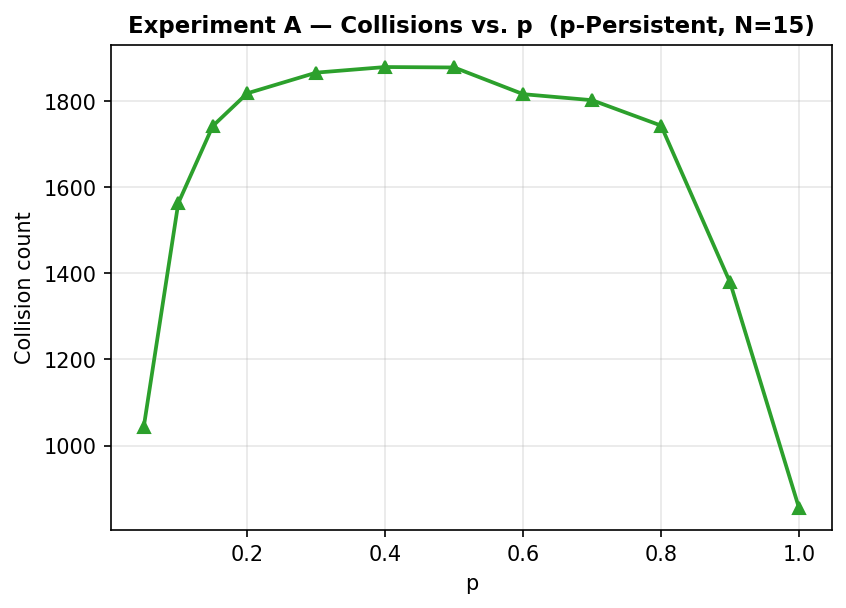
\includegraphics[width=0.85\textwidth]{figures/expA_collisions.png}
\caption{Collisions vs.\ $p$.}
\end{figure}
\begin{figure}[H]
\centering
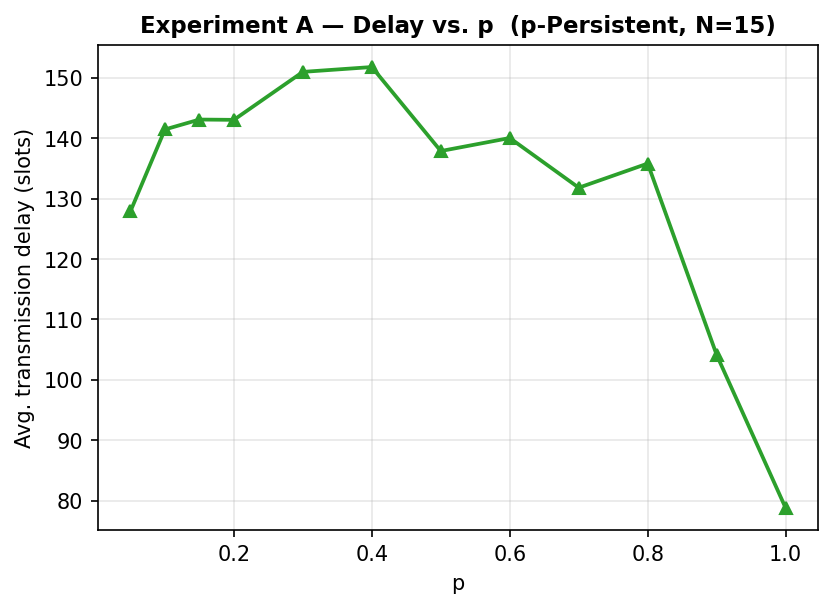
\includegraphics[width=0.85\textwidth]{figures/expA_delay.png}
\caption{Average transmission delay vs.\ $p$.}
\end{figure}
\begin{figure}[H]
\centering
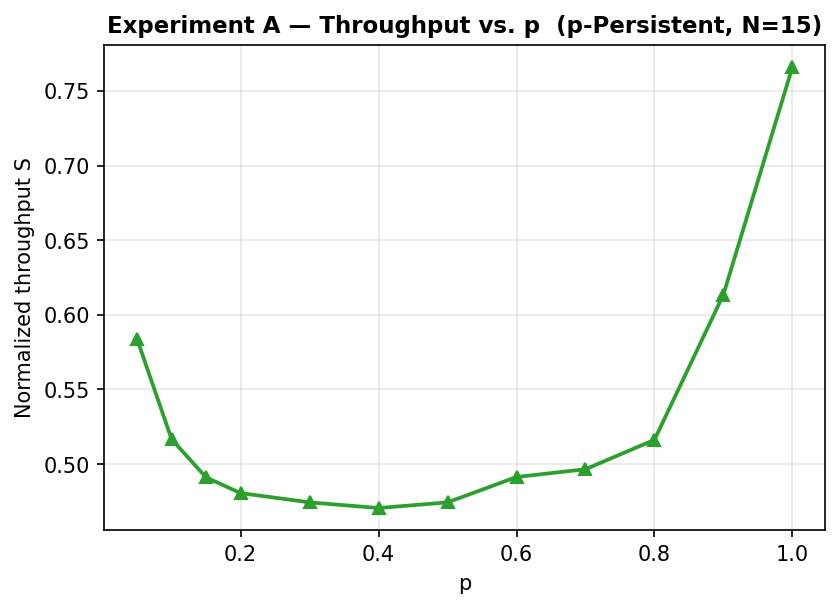
\includegraphics[width=0.85\textwidth]{figures/expA_throughput.png}
\caption{Normalized throughput vs.\ $p$.}
\end{figure}

\subsection{Experiment B --- All Schemes, Sweep $N$}
\label{sec:expB}
$p$-Persistent uses $p=1.0$, the best value found in Experiment A.

\begin{table}[H]
\centering
\small
\begin{tabular}{rrrrr}
\toprule
\textbf{N} & \textbf{Non-Pers.} & \textbf{1-Pers.} & \textbf{$p$-Pers. ($p{=}1$)} & \textbf{CSMA/CD} \\
\midrule
2   & 44   & 45   & 48   & 48 \\
5   & 192  & 194  & 211  & 196 \\
10  & 502  & 497  & 527  & 393 \\
15  & 877  & 795  & 942  & 649 \\
20  & 1489 & 1250 & 1217 & 764 \\
30  & 1846 & 1857 & 1888 & 1266 \\
40  & 2117 & 2182 & 2200 & 1790 \\
60  & 2523 & 2530 & 2493 & 2497 \\
80  & 2742 & 2697 & 2702 & 3152 \\
100 & 2853 & 2832 & 2847 & 3539 \\
\bottomrule
\end{tabular}
\caption{Experiment B --- Collisions vs.\ $N$.}
\end{table}

\begin{table}[H]
\centering
\small
\begin{tabular}{rrrrr}
\toprule
\textbf{N} & \textbf{Non-Pers.} & \textbf{1-Pers.} & \textbf{$p$-Pers. ($p{=}1$)} & \textbf{CSMA/CD} \\
\midrule
2   & 5.06    & 5.06    & 5.07    & 5.02 \\
5   & 6.09    & 9.92    & 11.07   & 8.54 \\
10  & 32.63   & 30.09   & 43.23   & 10.23 \\
15  & 58.13   & 54.18   & 77.77   & 27.96 \\
20  & 150.03  & 117.48  & 108.85  & 27.58 \\
30  & 261.03  & 254.21  & 257.07  & 90.13 \\
40  & 375.22  & 392.62  & 396.90  & 108.25 \\
60  & 737.42  & 710.53  & 745.48  & 266.38 \\
80  & 1110.99 & 995.76  & 1054.49 & 377.83 \\
100 & 1366.95 & 1360.60 & 1390.90 & 481.81 \\
\bottomrule
\end{tabular}
\caption{Experiment B --- Average transmission delay (slots) vs.\ $N$.}
\end{table}

\begin{table}[H]
\centering
\small
\begin{tabular}{rrrrr}
\toprule
\textbf{N} & \textbf{Non-Pers.} & \textbf{1-Pers.} & \textbf{$p$-Pers. ($p{=}1$)} & \textbf{CSMA/CD} \\
\midrule
2   & 0.9875 & 0.9872 & 0.9868 & 0.9960 \\
5   & 0.9470 & 0.9463 & 0.9417 & 0.9848 \\
10  & 0.8615 & 0.8642 & 0.8548 & 0.9700 \\
15  & 0.7542 & 0.7823 & 0.7408 & 0.9507 \\
20  & 0.5938 & 0.6610 & 0.6683 & 0.9423 \\
30  & 0.4995 & 0.5028 & 0.4920 & 0.9070 \\
40  & 0.4340 & 0.4198 & 0.4158 & 0.8632 \\
60  & 0.3392 & 0.3352 & 0.3458 & 0.8113 \\
80  & 0.2913 & 0.2970 & 0.2973 & 0.7632 \\
100 & 0.2635 & 0.2647 & 0.2617 & 0.7392 \\
\bottomrule
\end{tabular}
\caption{Experiment B --- Normalized throughput $S$ vs.\ $N$.}
\label{tab:throughputN}
\end{table}

\begin{figure}[H]
\centering
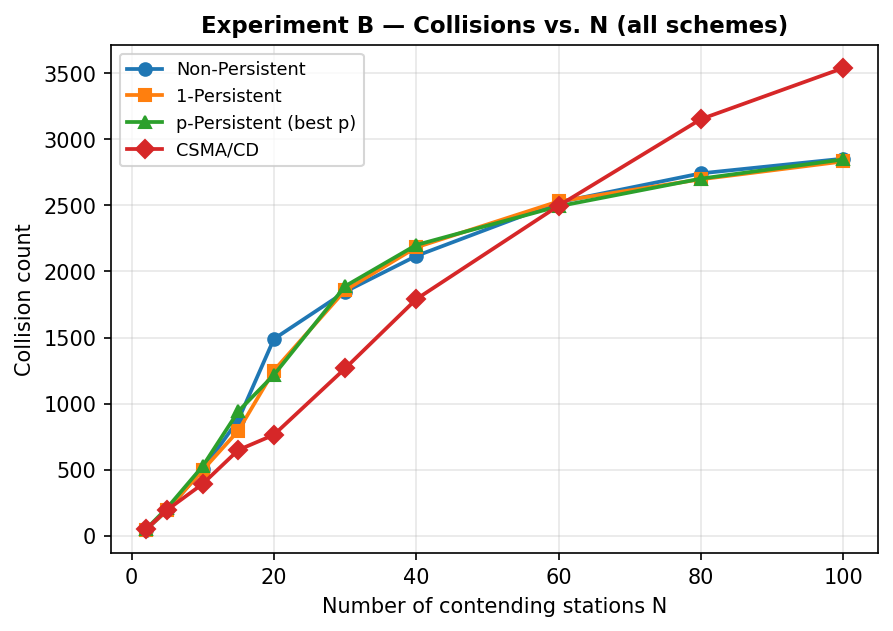
\includegraphics[width=0.85\textwidth]{figures/expB_collisions.png}
\caption{Collision count vs.\ $N$, all four schemes.}
\end{figure}
\begin{figure}[H]
\centering
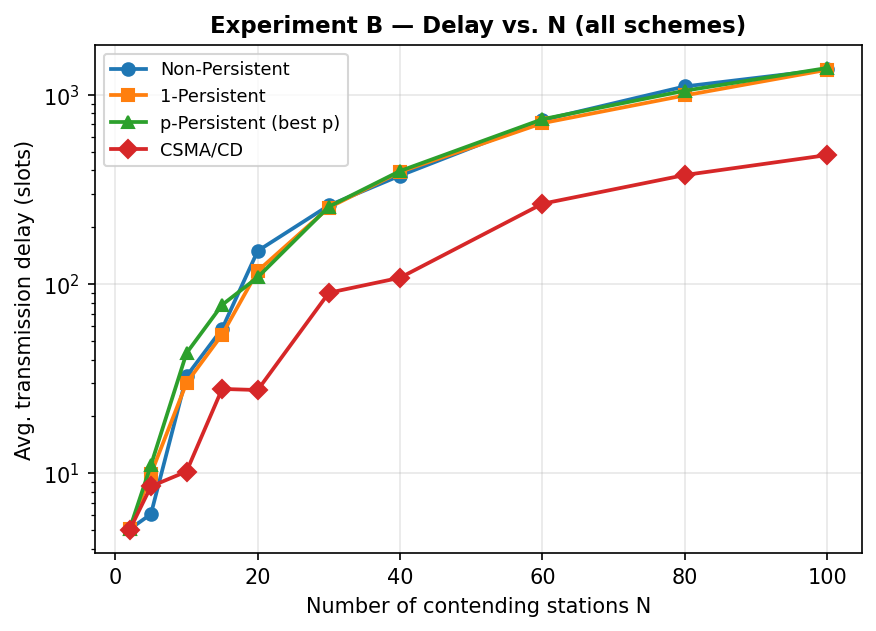
\includegraphics[width=0.85\textwidth]{figures/expB_delay.png}
\caption{Average transmission delay vs.\ $N$ (log scale), all four schemes.}
\end{figure}
\begin{figure}[H]
\centering
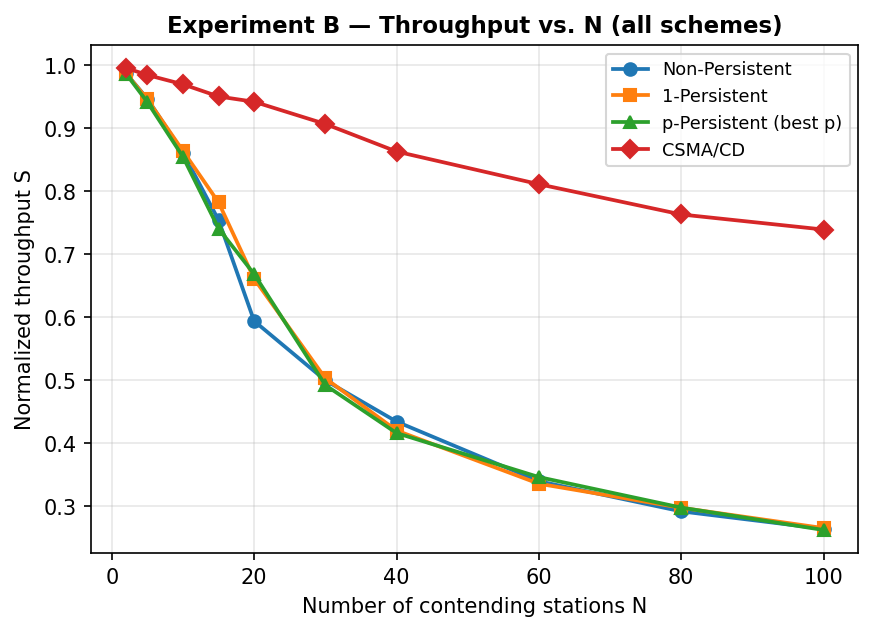
\includegraphics[width=0.85\textwidth]{figures/expB_throughput.png}
\caption{Normalized throughput vs.\ $N$, all four schemes.}
\end{figure}

\section{Analysis}

\subsection{Why throughput is U-shaped in $p$ (Experiment A)}
Table~\ref{tab:expA} shows throughput falling from 0.584 at $p{=}0.05$ to a minimum of
0.470 around $p{=}0.4$, then climbing back to 0.766 at $p{=}1.0$. Two competing costs
explain this:
\begin{itemize}[leftmargin=1.6em]
  \item \textbf{Low $p$:} a waiting station transmits with low probability on each idle
  slot, so it takes many idle slots, on average, before any of the 15 backlogged stations
  actually transmits. Collisions are rare (1044 at $p{=}0.05$, the lowest in the sweep) but
  the channel sits idle far more often (3110 idle slots out of 20000, also the sweep's
  maximum) --- caution wastes capacity.
  \item \textbf{Mid $p$ (0.3--0.5):} with 15 stations each independently flipping a coin
  near $p\approx1/N \approx 0.4$ would be the classical ALOHA-style optimum for a
  \emph{single-shot} decision, but because every waiting station re-flips on \emph{every}
  idle slot (not just once), the effective attempt rate compounds and collisions peak here
  (1879 at $p{=}0.4$, the sweep's maximum) rather than throughput.
  \item \textbf{High $p$ (up to 1.0):} once a slot is sensed idle, a station is now
  \emph{very} likely to seize it immediately, minimizing the idle-slot waste of low $p$.
  Collisions still happen (855 even at $p{=}1.0$) but the shared binary exponential backoff
  (\S2.2) resolves them efficiently enough that this regime wins overall --- at $p{=}1.0$,
  $p$-persistent's sensing rule is identical to 1-persistent's, and its throughput (0.766)
  is close to 1-persistent's own measurement at the same $N=15$ (0.782, Table~\ref{tab:throughputN}).
\end{itemize}
This is a different-shaped curve than the classical memoryless single-decision $p$-persistent
analysis (which typically shows a single peak at a moderate $p$ and degrades at $p\to1$
\emph{without} a backoff mechanism); the difference here is that all four schemes share the
same post-collision backoff, which specifically compensates for $p{=}1$'s otherwise-heavy
collision rate and lets it win.

\subsection{Why the three non-CD schemes converge, and why CSMA/CD pulls away (Experiment B)}
Table~\ref{tab:throughputN} and the throughput figure show Non-Persistent, 1-Persistent, and
$p$-Persistent tracking each other closely across the entire $N$ range (within a few
percentage points at every point), while CSMA/CD separates sharply once $N \ge 15$, ending at
0.739 vs.\ $\approx 0.26$ for the other three at $N=100$ --- a throughput advantage of
nearly $3\times$.

\paragraph{Why the non-CD schemes converge.} All three pay the identical cost for a
collision: the full \texttt{frameSlots}$=5$ duration is wasted before the sender even learns
the frame failed, and all three then recover via the same binary exponential backoff. The
only thing that differs between them is the idle-sensing rule, which affects \emph{how
quickly} a station notices the channel is free -- a second-order effect once the dominant
cost (collision duration) is identical. This is exactly the point of holding backoff
constant across schemes (\S2.2): it demonstrates that persistence strategy alone, without
collision detection, has limited leverage over saturation throughput.

\paragraph{Why CSMA/CD dominates -- and a counter-intuitive detail.} CSMA/CD's advantage is
not that it collides less often; Table~2 (Collisions vs.\ $N$) shows the \emph{opposite} at
high $N$ --- CSMA/CD has \emph{more} collision events than every other scheme at $N=80$
(3152 vs.\ $\approx$2700) and $N=100$ (3539 vs.\ $\approx$2850). What matters is that each of
those collisions costs only \texttt{jamSlots}$=1$ slot instead of \texttt{frameSlots}$=5$
slots -- a $5\times$ cheaper failure. Stations therefore cycle through failed attempts and
retry far faster, which is also why CSMA/CD's raw collision \emph{count} is higher: it
simply gets far more attempts into the same 20{,}000-slot window. Since each of those
attempts is cheap when it fails and the channel is freed almost instantly, CSMA/CD converts
that higher attempt rate into far more \emph{successes} too (2957 at $N=100$ vs.\ 1054--1059
for the other three) -- collision count alone is a misleading efficiency metric; the product
of collision frequency and collision cost is what determines throughput, and CSMA/CD wins on
the second factor by exactly the \texttt{frameSlots}/\texttt{jamSlots}$=5\times$ margin built
into the simulation parameters.

\subsection{Delay growth and saturation instability}
The delay-vs-$N$ figure (log scale) shows all four schemes' average delay growing roughly
two orders of magnitude from $N{=}2$ to $N{=}100$, with CSMA/CD's curve consistently an order
of magnitude below the other three past $N{=}20$. This is the classic saturation-instability
signature of contention-based MAC protocols: with every station permanently backlogged and
no admission control, once the offered attempt rate exceeds what the channel can resolve,
queueing delay grows superlinearly rather than the system settling into a stable
equilibrium. CSMA/CD pushes this effective ``capacity wall'' much further out (to a higher
$N$) purely by making each failed attempt cheap.

\subsection{A Bug Found and Fixed During Testing}
The first working version of \texttt{channel\_server} miscounted transmission duration by
exactly one slot per event: a new transmission's \emph{initiating} slot (the slot in which
the channel was sensed idle and a station decided to transmit) was never added to either the
idle-slot or the busy-duration tally, only the \texttt{frameSlots}$-1$ slots \emph{after} it
were. A first test run (5 stations, 1-persistent, 2000 slots, \texttt{frameSlots}$=5$)
showed successes$\times5$ + collisions$\times5$ + idle $= 1669$ against a horizon of 2000 --
331 slots unaccounted for, matching almost exactly the 330 transmission events in that run
(TC1). The fix moved the busy-until calculation to include the initiating slot itself
(\texttt{busyUntil = slot + frameSlots} rather than \texttt{slot + 1 + frameSlots}); after
the fix, every run in \S4 balances the slot-accounting identity exactly (modulo at most
\texttt{frameSlots}$-1$ slots from a transmission still in flight when the horizon is
reached).

\section{Comments}

\paragraph{Evaluation of the Lab Assignment.} Where Assignments 1 and 2 were about a single
sender/receiver pair behaving correctly, this assignment is fundamentally about \emph{many}
independent, uncoordinated decision-makers sharing one resource -- the interesting behavior
only emerges once $N>1$, and only becomes dramatic once $N$ is large enough that contention,
not raw capacity, is the bottleneck. Building all four schemes on one shared lock-step
channel simulator made the textbook CSMA trade-offs (persistence vs.\ idle waste, collision
frequency vs.\ collision cost) directly measurable on the same axes.

\paragraph{Difficulty and Learning Outcomes.} The hardest part was resisting the temptation
to let each protocol's post-collision recovery differ ``because that's more realistic'' --
holding backoff constant across all four schemes was what made the $N$-sweep results
actually interpretable (\S5.2), rather than conflating two different design choices into one
throughput number. The slot-accounting bug (\S5.3) was also instructive: it was invisible in
any single run's \emph{qualitative} behavior (successes, collisions, and throughput all
looked individually plausible) and only surfaced by explicitly checking the conservation
identity that total slots must be accounted for -- a reminder that a simulator can produce
believable-looking wrong numbers.

\paragraph{Suggested Improvements.} The delay metric, defined here as slots from
``frame ready'' to ``successfully delivered,'' conflates queueing delay (waiting for earlier
frames from the \emph{same} station) with contention delay (this specific frame's own
collisions and backoff); splitting them would make it possible to attribute delay growth
more precisely between the two. Running each configuration for several independent seeds and
averaging (as recommended for Assignment 2's Experiment B as well) would also smooth the
small non-monotonic wiggles visible in Table~\ref{tab:expA} between $p{=}0.4$ and $p{=}0.5$.

\end{document}
